随着项目的发展,在列表文件和源代码中查找内容变得越来越困难。因此,从一开始就保持项目的健康非常重要。

想象一下,您需要交付一些重要的、时间敏感的更改,而它们在项目的两个目录中都不适合。现在,需要快速地提交一个清理提交,该提交为文件引入更多的目录和另一层层次结构,以便更改可以有一个合适的位置。或者(更糟糕的是),你决定把它们扔到其他地方,然后手写一张便签,稍后再处理这个问题。

随着时间的推移,这些便签会累积起来,技术债务也会增加,维护代码的成本也会增加。当运行的系统中存在需要快速修复的严重缺陷时,当不熟悉代码库的开发者需要更改时,这就变得非常棘手。

所以,一个好的项目结构意味着什么呢?我们可以从软件开发的其他领域(例如,系统设计)借鉴一些规则。

项目应具备以下特点:

\begin{itemize}
\item 
易导航和扩展

\item 
自包含——例如,特定于项目的文件应该在项目目录中,而不在其他目录中。

\item 
抽象层次结构应该通过可执行文件和二进制文件来表示。
\end{itemize}

这里没有统一的解决方案,但在网上有很多可用的项目结构模板,我建议采用这个模板,因为其简单且易扩展:

\begin{center}
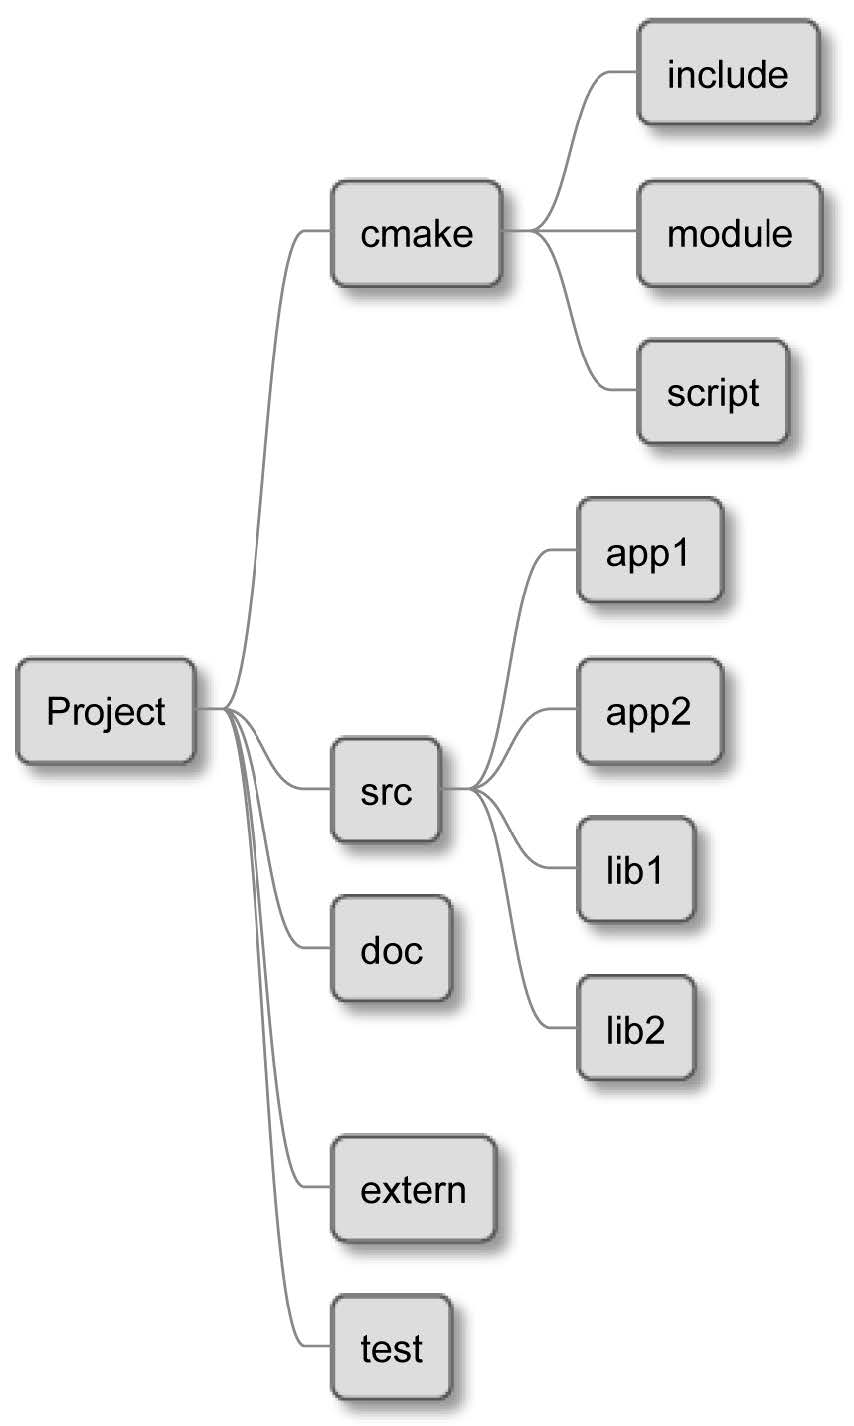
\includegraphics[width=0.5\textwidth]{content/1/chapter3/images/1.jpg}\\
图3.1 项目结构示例
\end{center}

本项目具有以下组件的目录:

\begin{itemize}
\item 
cmake: 宏和函数,查找模块和一次性脚本

\item 
src: 将存储的二进制文件和库的源代码

\item 
doc: 用于构建文档

\item 
extern: 从源代码构建的外部项目的配置

\item 
test: 包含自动测试的代码
\end{itemize}

这个结构中,CMakeLists.txt文件应该存在于以下目录中:顶级项目目录、src、doc、extern和test。主列表文件不应该自己声明构建步骤,应该使用add\_subdirectory()指令来执行嵌套目录中的所有列表文件。反之,可能会把这项工作委派给更深层。

\begin{tcolorbox}[colback=blue!5!white,colframe=blue!75!black,title=Note]
一些开发人员建议将可执行文件从库中分离出来,创建两个顶级目录而不是一个:src和lib。CMake对这两个工件一视同仁,在这个级别上的分离并不重要。
\end{tcolorbox}

src目录中拥有多个目录对于更大的项目来说非常方便,若只是构建一个可执行文件或库,可以跳过它们,直接将源文件存储在src中。因此,需要在那里添加一个CMakeLists.txt文件,并执行嵌套的列表文件。

这是文件树寻找单个目标的方式:

\begin{center}
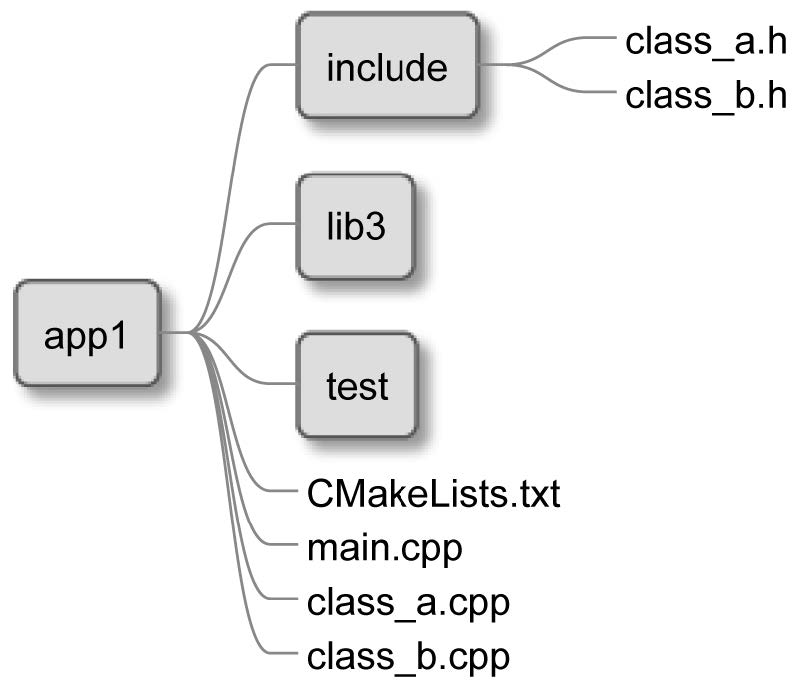
\includegraphics[width=0.5\textwidth]{content/1/chapter3/images/2.jpg}\\
图3.2 可执行文件的目录结构
\end{center}

在app1目录的根目录中看到一个CMakeLists.txt文件——配置关键项目设置,并包括来自嵌套目录的所有列表文件。src目录包含另一个CMakeLists.txt文件和.cpp实现文件:两个类和带有可执行文件入口点的主文件。CMakeLists.txt文件应该定义一个使用这些源文件构建可执行文件的目标——将在下一章学习如何做到这一点。

头文件在include目录中——.cpp实现文件使用这些文件来声明来自其他C++编译单元的符号。

我们有一个test目录来存放自动化测试的源码,还有lib3,只包含一个特定于这个可执行文件的库(在项目的其他地方使用的库或在它之外导出的库应该位于src目录中)。

这种结构非常有表现力,可以对项目进行许多扩展。随着类添加越来越多,可以很容易地将它们分组到库中,以加快编译过程。来看看库的目录结构:

\begin{center}
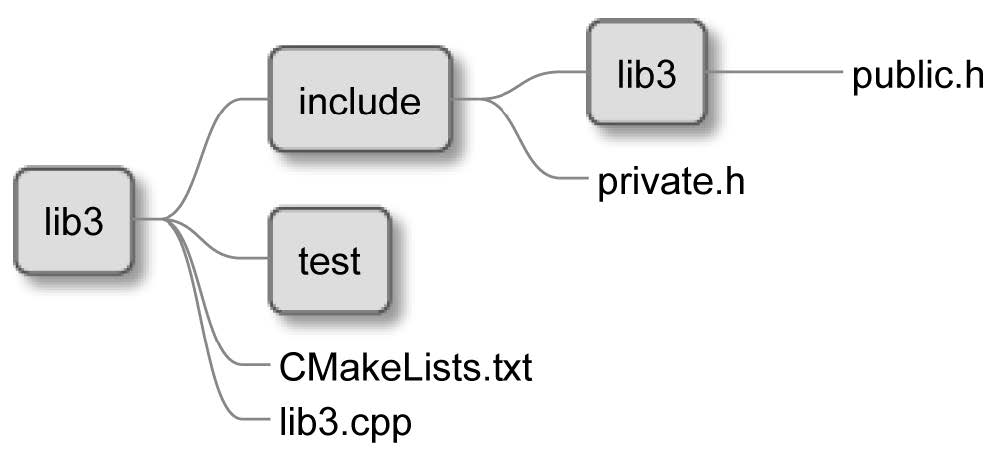
\includegraphics[width=0.6\textwidth]{content/1/chapter3/images/3.jpg}\\
图3.3 库的目录结构
\end{center}

库遵循与可执行文件相同的结构,只有很小的区别:include目录中有一个可选的lib3目录。只有当从项目外部使用库时,才会出现这种情况,其提供了其他项目在编译期间将使用的公共头文件。将在第5章开始构建自己的库时回到这个主题。

因此,已经讨论了如何在目录结构中布局文件。现在,来看看各个CMakeFiles.txt文件是如何组合在一起形成单个项目的,以及其在更大的场景中扮演什么角色。

\begin{center}
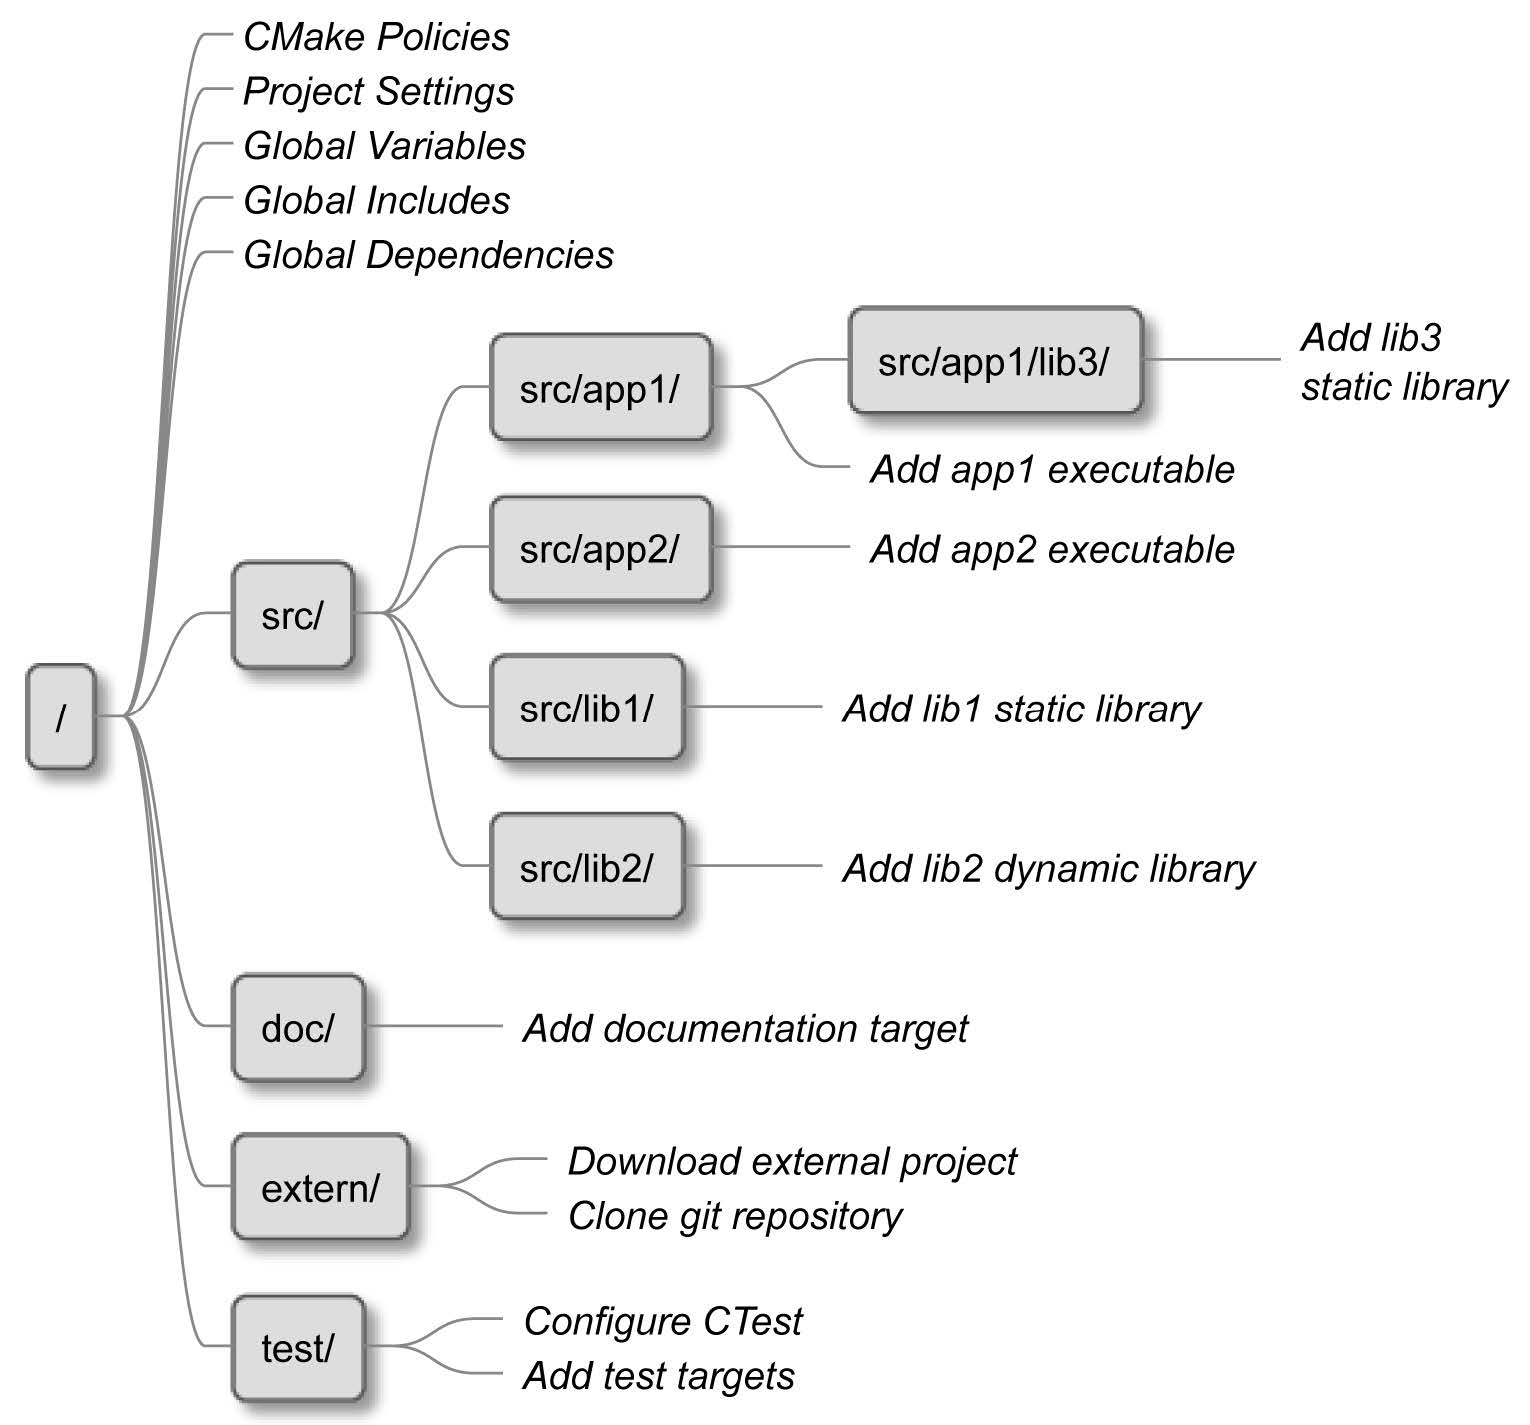
\includegraphics[width=0.8\textwidth]{content/1/chapter3/images/4.jpg}\\
图3.4 CMake如何在单个项目中合并列表文件
\end{center}

图3.4中,每个框表示驻留在给定目录中的CMakeLists.txt列表文件,而文本中的标签表示每个文件执行的操作(从上到下)。让我们再从CMake的角度来分析一下这个项目:

\begin{enumerate}
\item 
执行从项目的根开始——从源码树中的列表文件开始。该文件将使用适当的策略设置最低要求的CMake版本,设置项目名称、支持的语言、全局变量,并包括来自CMake目录的文件,以便内容全局可用。

\item 
下一步是通过使用add\_subdirectory(src bin)指令进入src目录的范围(将编译好的工件放在<binary\_tree>/bin,而不是<binary\_tree>/src)。

\item 
CMake读取src/CMakeLists.txt文件,发现其唯一用途是添加四个嵌套子目录:app1、app2、lib1和lib2。

\item 
CMake进入app1的变量作用域,了解另一个嵌套库lib3,有自己的CMakeLists.txt文件;然后输入lib3的作用域。

\item 
lib3库添加了一个具有相同名称的静态库目标。CMake返回app1的父范围。

\item 
app1子目录添加了一个依赖于lib3的可执行文件。CMake返回src的父范围。

\item 
CMake将继续进入剩下的嵌套作用域并执行它们的列表文件,直到完成所有add\_subdirectory()。

\item 
CMake返回到顶级作用域并执行剩下的三个指令:add\_subdirectory(doc)、add\_subdirectory(extern)和add\_subdirectory(test)。CMake每次都进入新的作用域,并从适当的列表文件执行指令。

\item 
收集所有的目标并检查其正确性,CMake现在拥有生成构建系统所需的所有信息。
\end{enumerate}

前面步骤的发生顺序与列表文件中写入命令的顺序完全一致。有时这很重要,而另一些时候则不是那么重要。我们将在下一章深入探讨。

那么,什么时候是创建目录以包含项目的所有元素的最佳时间呢?应该从一开始就做正确的事情——创建未来需要的所有东西,并保持目录为空——还是等到我们真正有了需要归入自己类别的文件?这是一种选择——可以遵循极限编程规则YAGNI(不需要它),或者可以尝试让项目具有前瞻性,为接纳新开发人员的到来奠定良好的基础。

试着在这些方法之间取得良好的平衡——若怀疑项目有一天可能需要extern目录,那么就添加它(可能需要创建一个空的.keep文件来将目录检入存储库)。为了帮助其他人知道在哪里放置他们的外部依赖项,创建一个自述文件,并为未来将走上这条路的缺乏经验的程序员铺平道路。您可能已经注意到:开发人员不愿意创建目录,特别是在项目的根目录中。若提供一个好的项目结构,人们会倾向于遵循它。

有些项目可以在几乎所有的环境中构建,而另一些项目则对其细节非常挑剔。顶层列表文件是评估如何进行项目的最佳位置,这取决于可用的内容。





